% \documentclass[12pt]{article}

%%v helpful MIT exam schema, see http://www-math.mit.edu/~psh/exam/examdoc.pdf
 \documentclass[12pt]{exam} 
% \qformat{\textbf{Question \thequestion}\quad \thepoints\hfill } % Large depth to make space}
 \renewcommand{\thesubpart}{(\roman{subpart})}
 \renewcommand{\subpartlabel}{\thesubpart}
 \footer{}{}{Page \thepage\ de \numpages}
\addpoints
\pointsinmargin
% \boxedpoints
\renewcommand{\questionshook}{\setlength{\itemsep}{1mm}}
\renewcommand{\partshook}{
	\setlength{\itemsep}{0.1cm}
}

\usepackage{cmbright}
\pagestyle{empty} %for handouts
\addtolength{\jot}{2em} % this makes all formulae a bit more spaced vertically for handouts
\setlength{\parindent}{0pt} %we're not writing a novel
%\renewcommand{\arraystretch}{2} %makes tables taller, so easier to write in

\usepackage[fleqn]{amsmath}
\usepackage{amssymb} %standard classy maths symbols
\usepackage[a4paper, margin=1in]{geometry} %makes it easy to specify where to put stuff on the page

\usepackage{siunitx} %v handy way of getting SI units to typeset correctly...
% \sisetup{locale = FR} %... and now it will use a comma for decimals

\usepackage[utf8]{inputenc}

% \usepackage[french]{babel} % frenchify everything (e.g. a Table becomes a Tableau)
% \usepackage{lmodern} % font with nicer French characters than standard
% \usepackage{textcomp} % and more help for special characters

\usepackage{tcolorbox} % basic but good package for boxes around text
\tcbset{colback=black!5!white}
% \usepackage{color} % colours
%\newcommand{\fillin}{\color{black!1!white}} %makes the text disappear
%\definecolor{fillin}{rgb} {1.00,1.00,1.00}
%\renewcommand{\fillin}{\color{blue}} \definecolor{fillin}{rgb} {0.00,0.00,1.00} %makes the filling in text appear (in blue)

\usepackage{enumitem} % can change the labels on lists, items, enumerates
\usepackage{setspace}

%\usepackage{tikz, pgfplots} % interval diagrams, sets, etc.
%\usetikzlibrary{calc,trees,positioning,arrows,fit,shapes}
\usepackage{graphicx}

\usepackage{letltxmacro}
\makeatletter
\let\oldr@@t\r@@t
\def\r@@t#1#2{%
\setbox0=\hbox{$\oldr@@t#1{#2\,}$}\dimen0=\ht0
\advance\dimen0-0.2\ht0
\setbox2=\hbox{\vrule height\ht0 depth -\dimen0}%
{\box0\lower0.4pt\box2}}
\LetLtxMacro{\oldsqrt}{\sqrt}
\renewcommand*{\sqrt}[2][\ ]{\oldsqrt[#1]{#2}}
\makeatother

\begin{document}

\textbf{Name:} \dotfill

\begin{questions}

\question[6] Circle the monomials in the following algebraic expressions 
$$ 5 \hspace{10mm} \pi x^2 \hspace{10mm} -7x^{-2} \hspace{10mm} (5 + x) \hspace{10mm} \sqrt{7} x \hspace{10mm} \sqrt{7x}$$



\fullwidth{Let $P(x) = x^3 + 3x + 5$ and $Q(x) = x^2 -3$.}

\question[2] Calculate the sum $(P + Q)(x)$. \\
\emph{This means calculate $P(x) + Q(x)$.}
\fillwithdottedlines{14mm}
\question[4] Calculate the product $(P \cdot Q)(x)$. \\
\emph{This means calculate $P(x) \cdot Q(x)$.}
\fillwithdottedlines{35mm}
\question[4] What are the degrees of $P$, $Q$, $P+Q$ and $P \cdot Q$ ?
\fillwithdottedlines{14mm}
\question[3] Calculate $Q(x)^3$
\fillwithdottedlines{35mm}

\question[2] Without doing the algebra, determine the degree of $(x^2 + 76x + 91)^{50}$.
\fillwithdottedlines{14mm}


\vfill

\end{questions}

\begin{tcolorbox}

\textbf{Name of correcter:}
\begin{center}
\gradetable[h][questions]
\end{center}

\end{tcolorbox}

\newpage

\textbf{Pascal's Triangle}

One of the most interesting Number Patterns is Pascal's Triangle (named after Blaise Pascal, a famous French Mathematician and Philosopher).

\

To build the triangle, start with "1" at the top, then continue placing numbers below it in a triangular pattern. Each number is the numbers directly above it added together.
\vspace{-3mm}
\begin{center}
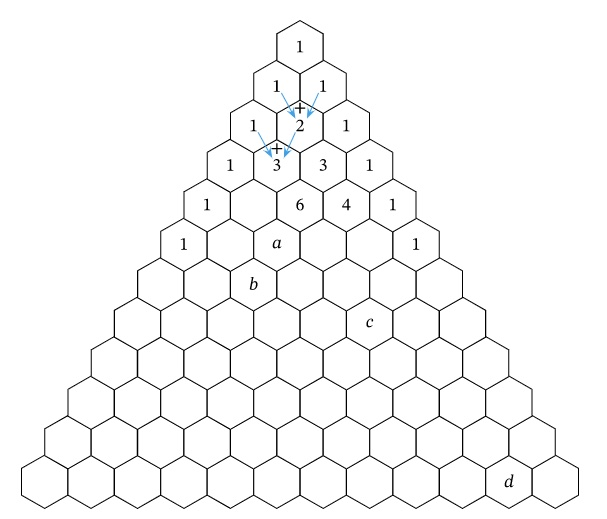
\includegraphics[width=0.7\textwidth]{pascaltriangle.jpg}
\end{center}

By spotting patterns, or otherwise, find the values of $a$, $b$, $c$ and $d$.
$$a =  \qquad b = \qquad c= \qquad d= $$
\

Now expand and simplify the following polynomials:

\vspace{8mm}

$(x+1)^1 = $

\vspace{8mm}

$(x+1)^2 = $

\vspace{12mm}

$(x+1)^3 = $

\vspace{12mm}

$(x+1)^4 = $

\vspace{12mm}

What do you notice? Use Pascal's Triangle to calculate $(x+1)^{8}$.
\end{document}